

\documentclass[12pt]{letter}

\usepackage[margin=1in,footskip=0.25in]{geometry}
\usepackage{amsfonts}
\usepackage{amsthm}
\usepackage{pgf}
\usepackage{tikz}
\usepackage{amsmath}
\usetikzlibrary{arrows,automata}
\usetikzlibrary{positioning}
\usepackage[latin1]{inputenc}
\tikzset{>=latex}
\newcommand\tab[1][2cm]{\hspace*{#1}}

\begin{document}
Class: COMP 3040 - Foundation of Computer Science \\ Name: DangNhi Ngoc Ngo \\ Student ID: 01553277 \\ Homework 3

\centering\textbf{Homework 3: Chapter 2 - CFG, PDA}

\flushleft


\begin{enumerate}
\item[\textbf{2.1}]Recall the CFG $G_4$ that we gave in Example 2.4. For convenience, let's rename its variables with single letters as follows.

\setlength\parindent{150pt}
$E \rightarrow E + T \mid T $ \\
$T \rightarrow T \times F \mid F $ \\
$F \rightarrow (E)  \mid  a$ \\  \setlength\parindent{0pt}
\leavevmode \\

Give parse trees and derivations of each string.
\begin{enumerate}
	\item[\textbf{a}.] a \\
	The derivation is $E \Rightarrow T \Rightarrow F \Rightarrow a.$
	\begin{center}
	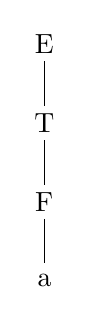
\begin{tikzpicture}[state/.style={inner sep=0pt, minimum size=12pt},node distance=1cm, on grid, auto] 
		\node[state] (q0) {E};
		\node[state] (q1) [below= of q0] {T};
		\node[state] (q2)[below= of q1]  {F};
		\node[state] (q3)[below= of q2]  {a};
		\path[-] 
			(q0) edge node {} (q1)
			(q1) edge node {} (q2)
			(q2) edge node {} (q3);
	\end{tikzpicture}
	\end{center}

	\item[\textbf{b}.] $a + a$ \\
	The derivation is $E \Rightarrow E + T \Rightarrow T + T \Rightarrow F + T \Rightarrow a + T \Rightarrow a + F \Rightarrow a + a.$
	\begin{center}
	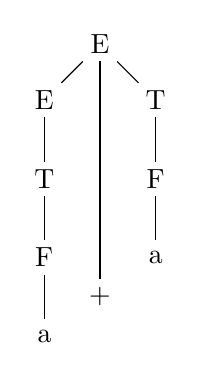
\begin{tikzpicture}[state/.style={inner sep=0pt, minimum size=12pt},node distance=1cm, on grid, auto] 
		\node[state] (q0) {E};
		\node[state] (q1) [below left=of q0] {E};
		\node[state] (q2)[below=of q1]  {T};
		\node[state] (q3)[below=of q2]  {F};
		\node[state] (q4)[below=of q3]  {a};
		\node[state] (q5)[below=3.2cm of q0]  {$+$};
		\node[state] (q6)[below right=of q0]  {T};
		\node[state] (q7)[below=of q6]  {F};
		\node[state] (q8)[below=of q7]  {a};
		\path[-] 
			(q0) edge node {} (q1) edge node {} (q5) edge node {} (q6)
			(q1) edge node {} (q2)
			(q2) edge node {} (q3)
			(q3) edge node {} (q4)
			(q6) edge node {} (q7)
			(q7) edge node {} (q8);
	\end{tikzpicture}
	\end{center}
	\newpage

	\item[\textbf{c}.] $a + a + a$ \\
	The derivation is $E \Rightarrow E + T \Rightarrow E + T + T \Rightarrow T + T + T \Rightarrow F + T + T \Rightarrow a + T+ T \Rightarrow a + F + T \Rightarrow a + a + T \Rightarrow a + a+ F \Rightarrow a + a+ a.$
	\begin{center}
	\begin{tikzpicture}[state/.style={inner sep=0pt, minimum size=12pt},node distance=1cm, on grid, auto] 
		\node[state] (q0) {E};
		\node[state] (q1) [below left=2cm of q0] {E};
		\node[state] (q2) [below left=of q1] {E};
		\node[state] (q3) [below=of q2] {T};
		\node[state] (q4) [below=of q3] {F};
		\node[state] (q5) [below=of q4] {a};
		\node[state] (q6) [below=3.4cm of q1] {$+$};
		\node[state] (q7) [below right =of q1] {T};
		\node[state] (q8) [below=of q7] {F};
		\node[state] (q9) [below=of q8] {a};
		\node[state] (q10) [below=4cm of q0] {$+$};
		\node[state] (q11) [below right=2cm of q0] {T};
		\node[state] (q12) [below=of q11] {F};
		\node[state] (q13) [below=of q12] {a};
		\path[-] 
			(q0) edge node {} (q1) edge node {} (q11) edge node {} (q10)
			(q1) edge node {} (q2) edge node {} (q6) edge node {} (q7)
			(q2) edge node {} (q3)
			(q3) edge node {} (q4)
			(q4) edge node {} (q5)
			(q7) edge node {} (q8)
			(q8) edge node {} (q9)
			(q11) edge node {} (q12)
			(q12) edge node {} (q13);
	\end{tikzpicture}
	\end{center}

	\item[\textbf{d}.] $((a))$ \\
	The derivation is $E \Rightarrow T \Rightarrow F \Rightarrow (E) \Rightarrow (T) \Rightarrow (F) \Rightarrow ((E)) \Rightarrow ((T)) \Rightarrow ((F)) \Rightarrow ((a))   $
	\begin{center}
	\begin{tikzpicture}[state/.style={inner sep=0pt, minimum size=12pt},node distance=1cm, on grid, auto] 
		\node[state] (q0) {E};
		\node[state] (q1) [below= of q0] {T};
		\node[state] (q2) [below= of q1] {F};
		\node[state] (q3) [below= of q2] {E};
		\node[state] (q4) [below= of q3] {T};
		\node[state] (q5) [below= of q4] {F};
		\node[state] (q6) [below= of q5] {E};
		\node[state] (q7) [below= of q6] {T};
		\node[state] (q8) [below= of q7] {F};
		\node[state] (q9) [below= of q8] {a};
		\node[state] (q10) [left= 2cm of q6] {$($};
		\node[state] (q11) [right= 2cm of q6] {$)$};
		\node[state] (q12) [left= 1.5cm of q9] {$($};
		\node[state] (q13) [right= 1.5cm of q9] {$)$};
		\path[-] 
			(q0) edge node {} (q1)
			(q1) edge node {} (q2)
			(q2) edge node {} (q3) edge [bend right] node {} (q10)  edge [bend left] node {} (q11)
			(q3) edge node {} (q4)
			(q4) edge node {} (q5)
			(q5) edge node {} (q6)
			(q6) edge node {} (q7) edge [bend right] node {} (q12)  edge [bend left] node {} (q13)
			(q7) edge node {} (q8)
			(q8) edge node {} (q9);
	\end{tikzpicture}
	\end{center}
\end{enumerate}

\ \\ % create a new line
\item[\textbf{2.4}]Give context-free grammars that generate the following languages. In all parts, the alphabet  $\sum$ is $\{0,1\}$.
\begin{enumerate}
	\item[\textbf{b}.] $\{ w \mid w$ starts and ends with the same symbol$\}$
	\leavevmode \\
	$S \rightarrow 0R0 \mid 1R1 \mid \varepsilon$ \\
	$R \rightarrow 0R \mid 1R \mid \varepsilon$ \\

	\leavevmode \\
	\item[\textbf{c}.] $\{ w \mid $the length of w is odd$\}$
	\leavevmode \\
	$S \rightarrow 0 \mid 1 \mid 00S \mid 01S \mid 10S \mid 11S$ \\

	\leavevmode \\
	\item[\textbf{e}.] $\{ w \mid w^R$, that is, $w$ is a palindrome$\}$
	\leavevmode \\
	$S \rightarrow B1B$ \\
	$B \rightarrow BB \mid 0B1 \mid 1B0 \mid 1 \mid \varepsilon$ \\
	$S$ forces an extra 1, because $B$ creates strings that satisfy to have at least as many 1s as 0s

	\leavevmode \\
	\item[\textbf{f}.] The empty set
	\leavevmode \\
	$S \rightarrow S$ \\

\end{enumerate}

\ \\ % create a new line
\item[\textbf{2.5}] Give informal descriptions and state diagrams of pushdown automate for the language in Exercise 2.4.
\begin{enumerate}
	\item[\textbf{b}.] $\{ w \mid w$ starts and ends with the same symbol$\}$
	\leavevmode \\
	Informal Description: \\
	If the string has only one symbol (by nondeterministically guessing), we can accept it without using the stack.\\
	Otherwise, pushing the first symbol read into the stack, then reading every other symbol and guessing if that is the last symbol read. \\
	We can accept in the case the last symbol read matches with the symbol in the stack and no more input. If not, we reject it.

\ \\ % create a new line
	\leavevmode \\
	State diagrams: \\
	\begin{center}
	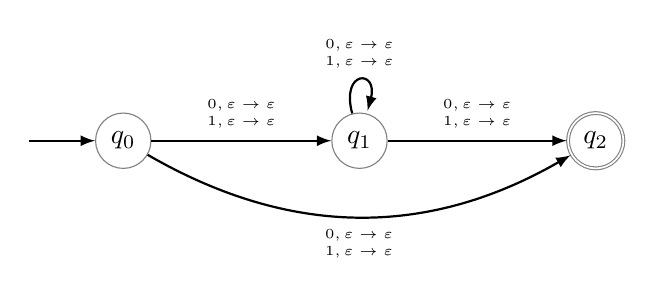
\begin{tikzpicture}[state/.style={circle, draw=black!50, inner sep=0pt, minimum size=20pt},node distance=3cm, on grid, auto] 
		\node[state] (q0) {$q_0$};++
		\node[state] (q1) [right= of q0] {$q_1$};
		\node[state, accepting] (q2) [right=of q1] {$q_2$};
		\draw[<-, thick] (q0) -- ++(-1.2cm,0);
		\path[->,thick] 
			(q0) edge node {\tiny\begin{tabular}{c}$0,\varepsilon \rightarrow \varepsilon$ \\ $1,\varepsilon \rightarrow \varepsilon$ \end{tabular}} (q1)  edge [bend right] node [below] {\tiny\begin{tabular}{c}$0,\varepsilon \rightarrow \varepsilon$ \\ $1,\varepsilon \rightarrow \varepsilon$ \end{tabular}} (q2)
			(q1) edge node {\tiny\begin{tabular}{c}$0,\varepsilon \rightarrow \varepsilon$ \\ $1,\varepsilon \rightarrow \varepsilon$ \end{tabular}} (q2) edge [loop above] node {\tiny\begin{tabular}{c}$0,\varepsilon \rightarrow \varepsilon$ \\ $1,\varepsilon \rightarrow \varepsilon$ \end{tabular}} (q1);
	\end{tikzpicture}
	\end{center}
\newpage

	\item[\textbf{c}.] $\{ w \mid $ the length of $w$ is odd$\}$
	\leavevmode \\
	Informal Description: \\
	In this case, we do not need to use the stack.\\
	We can read the input and only accept if the length is odd, that is after the first symbol read or every other symbol read thereafter if it is the final symbol read. \\
	\leavevmode \\
	State diagrams: \\
	\begin{center}
	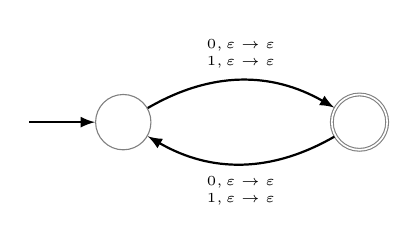
\begin{tikzpicture}[state/.style={circle, draw=black!50, inner sep=0pt, minimum size=20pt},node distance=3cm, on grid, auto] 
		\node[state] (q0) {};
		\node[state, accepting] (q1) [right=of q0] {};
		\draw[<-, thick] (q0) -- ++(-1.2cm,0);
		\path[->,thick] 
			(q0) edge [bend left] node {\tiny\begin{tabular}{c}$0,\varepsilon \rightarrow \varepsilon$ \\ $1,\varepsilon \rightarrow \varepsilon$ \end{tabular}} (q1)
			(q1) edge [bend left] node {\tiny\begin{tabular}{c}$0,\varepsilon \rightarrow \varepsilon$ \\ $1,\varepsilon \rightarrow \varepsilon$ \end{tabular}} (q0);
	\end{tikzpicture}
	\end{center}


	\item[\textbf{e}.] $\{ w \mid w^R$, that is, $w$ is a palindrome$\}$
	\leavevmode \\
	Informal Description: \\
	In this case, we use the stack to push the symbols read into it.\\
	We can use the nondeterministically guess if the middle of the string has been reached, or if the next symbol read is the middle of the string and will not be put in the stack.\\
	If they match the input symbols read, we will pop the symbols out of the stack.
	In addition, if the stack empties as the input are finished, and the symbols popped are the same with the symbols that were pushed before, we will accept.
Otherwise, we reject it.\\

	\leavevmode \\
	State diagrams: \\ 
	\begin{center}
	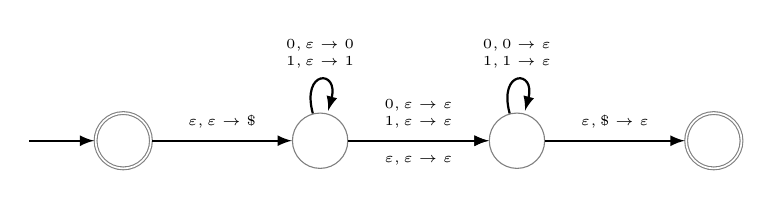
\begin{tikzpicture}[state/.style={circle, draw=black!50, inner sep=0pt, minimum size=20pt},node distance=2.5cm, on grid, auto] 
		\node[state,accepting] (q0) {};
		\node[state] (q1) [right=of q0] {};
		\node[state] (q2) [right=of q1] {};
		\node[state, accepting] (q3) [right=of q2] {};
		\draw[<-, thick] (q0) -- ++(-1.2cm,0);
		\path[->,thick]
			(q0) edge node {\tiny\begin{tabular}{c}$\varepsilon, \varepsilon \rightarrow \$ $ \end{tabular}} (q1)
			(q1) edge [loop above] node {\tiny\begin{tabular}{c}$0,\varepsilon \rightarrow 0$ \\ $1,\varepsilon \rightarrow 1$ \end{tabular}} (q1) edge node {\tiny\begin{tabular}{c}$0,\varepsilon \rightarrow \varepsilon$ \\ $1,\varepsilon \rightarrow \varepsilon$ \end{tabular}} (q2)  edge node [below] {\tiny\begin{tabular}{c}$\varepsilon,\varepsilon \rightarrow \varepsilon$ \end{tabular}} (q2)
			(q2) edge [loop above] node {\tiny\begin{tabular}{c}$0,0 \rightarrow \varepsilon$ \\ $1,1 \rightarrow \varepsilon$ \end{tabular}} (q2) edge node {\tiny\begin{tabular}{c}$\varepsilon,  \$ \rightarrow \varepsilon$ \end{tabular}} (q3);
	\end{tikzpicture}
	\end{center}

	\leavevmode \\
	\item[\textbf{f}.] The empty set
	\leavevmode \\
	Informal Description: \\
	The PDA consists of one state that does not accept.\\
	The CFG can not accept any strings, including the empty because there is no derivations terminating. \\
	\leavevmode \\
	State diagrams: \\ 
	\begin{center}
	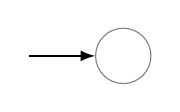
\begin{tikzpicture}[state/.style={circle, draw=black!50, inner sep=0pt, minimum size=20pt},node distance=2.5cm, on grid, auto] 
		\node[state] (q0) {};
		\draw[<-, thick] (q0) -- ++(-1.2cm,0);
	\end{tikzpicture}
	\end{center}
\end{enumerate}

\newpage
\item[\textbf{2.6}] Give context-free grammars generating the following languages.\\
\begin{enumerate}
	\item[\textbf{b}.] The complement of the language \{$a^nb^n \mid n \geq $0\}
	\leavevmode \\
	Rewrite the complement as: \\
	\begin{center} $\{a^nb^m$ : $ n \neq m\} \cup \{(a\cup b)^*ba(a \cup b)^*\}$\end{center}
	\ \\ % create a new line
	$L_1$ is the leftmost language. \\
	$L_2$ is the rightmost language. \\

	The context-free grammar that generate $L_1$ is: \\
	\setlength\parindent{100pt} 
	$S_1 \rightarrow aS_1b \mid T \ U$ \\
	$T \rightarrow aT \mid a$ \\
	$U \rightarrow Ub \mid b$
	\setlength\parindent{0pt} 

  The context-free grammar that generate $L_1$ is: \\
	\setlength\parindent{100pt} 
	$S_2 \rightarrow RbaR$ \\
	$R \rightarrow \mid a \mid b \mid \varepsilon$\\
	\setlength\parindent{0pt} 
	So, the final context-gree grammar G that generate $L_1 \cup L_2$ is: \\
	\leavevmode \\
	\setlength\parindent{100pt} 
	$S \rightarrow T \mid aU \mid Vb $\\
	$T \rightarrow aT \mid Ta \mid bT \mid Tb \mid ba$ \\
	$U \rightarrow aU \mid W$\\
	$V \rightarrow Vb \mid W$\\
	$W \rightarrow aWb \mid \varepsilon$\\
	\setlength\parindent{0pt} 


	\item[\textbf{d}.] $\{ x_1\#x_2\#...\#x_k \mid k \geq1$, each $x_i \in \{a,b\}^*$, and for some $i$ and $j$, $x_i = x_i^R\}$
	\leavevmode \\
	Rewrite: \\
	\begin{center} $...\#...\#w\#...\#w^R\#...\#...$\end{center}
	\leavevmode \\
	Let A be a non-terminal that generates $\{a, b, \#\}^*$, i.e.\\
	\leavevmode \\
	\begin{center} $A \rightarrow aA \mid bA \mid \#A \mid \varepsilon$\end{center}
	Then, the part $w\#...\#w^R$ can be generated as follows.\\
	\leavevmode \\
	\begin{center} $B \rightarrow aBa \mid bBb \mid \# \mid \#A\#$\end{center}
	\leavevmode \\
	The context-free grammars that generates is as follows: \\
	\leavevmode \\
	\setlength\parindent{100pt} 
	$S \rightarrow A\#B\#A \mid B\#A \mid A\#B \mid B$\\
	$B \rightarrow aBa \mid bBb \mid \# \mid \#A\#$ \\
	$A \rightarrow aA \mid bA \mid \#A \mid \varepsilon$
	\setlength\parindent{0pt} 
\end{enumerate}

\newpage
\item[\textbf{2.9}] Give a context-free grammar that generates the language.\\
\begin{center} $A = \{a^ib^jc^k \mid i = j or j = k$ where $i, j, k \geq 0 \}$. \end{center}
\leavevmode \\  \leavevmode \\ 
 Is your grammar ambigous? Why or why not? \\
\leavevmode \\
Rules: \\
\tab $S\:\rightarrow\:U\:|\:V$ \\
\tab $U\:\rightarrow\:aU\:|\:X$ \\
\tab $V\:\rightarrow\:Vc\:|\:Y$ \\
\tab $X\:\rightarrow\:bXc\:|\:\varepsilon$ \\
 \tab $Y\:\rightarrow\:aYb\:|\:\varepsilon$ \\ 
\leavevmode \\ 
 The grammar is ambiguous because we can have these two derivations. \\ 
\begin{center}
	\begin{tikzpicture}[tlabel/.style={pos=0.4,right=-1pt,font=\footnotesize\color{red!70!black}}]
	\node{S} 
		child { node{U} 
			child { node{a} }
				child { node{U}
					child { node{X}
						child { node{b} 
						}
						child { node{X} 
							child { node{$\varepsilon$} 
							}
						}
 						child {node{c} 
					}
				}
			}
               	 };
	\end{tikzpicture}
	\begin{tikzpicture}[tlabel/.style={pos=0.4,right=-1pt,font=\footnotesize\color{red!70!black}}]
	\node{S}
		child { node{V} 
			child { node{V} 
				child { node{Y}
					child { node{a} 
					}
				child { node{Y}
                                		child { node{$\varepsilon$}
					}
                           		}
                           		 child { node{b} 
				}
			}
		}
                   		child { node{c} 
			}
               	};
        \end{tikzpicture}
\end{center}

\ \\ % create a new line
\item[\textbf{2.10}] Give an informal description of a pushdown automaton that recognizes the language $A$ in Exercise 2.9.
\leavevmode \\ 
Informal description of a pushdown automaton that recognizes the langauge $A$.\\
\begin{itemize}
	\item Nondeterministically branch to step 2 or step 6.
	\item Read and push a's.
	\item Read b's, while popping a's out of the stack.
	\item Skip c's on input and $accept$ in the case b's finish when stack is empty.
	\item Skip a's on input.
	\item Read and push b's.
	\item Read c's, while popping b's out of the stack.
	\item $Accept$ if c's finish when stack is empty.
\end{itemize}
\leavevmode \\ 

\ \\ % create a new line
\item[\textbf{2.11}] Convert the CFG $G_4$ given in Exercise 2.1 to an equivalent PDA, using the procedure given in Theorem 2.20.\\
\setlength\parindent{150pt} $E \rightarrow E + T \mid T $ \\ $T \rightarrow T \times F \mid F $ \\ $F \rightarrow (E)  \mid  a$ \\  \setlength\parindent{0pt}
\leavevmode \\
	 The formal definition of the equivalent PDA =	(Q, $\Sigma$, $\Gamma$, $\delta$, q$_{1}$, F) where" \\
	Q = \{q$_{1}$,q$_{2}$\}; $\Sigma$ = \{+, x, (, ), a\}\\$\Gamma$ = \{E, T, F\} $\cup$ $\Sigma$; F = \{q$_{2}$\}.\\
	The transition function $\delta$: Q x $\Sigma _{\varepsilon}$ x $\Gamma_{\varepsilon} \longrightarrow$ P(Q X $\Gamma_{\varepsilon}$)\\
	\[   
	\delta(q,x,y) = 
	\begin{cases}
	\text{\{(q$_{2}, \varepsilon$)\}} 
	&\quad\text{if q = q$_{1}$, x = $\varepsilon$}, y =  $\textdollar$ \\
	
	\text{\{(q$_{1}, E+T$), (q$_{1}$, T)\}} 
	&\quad\text{if q = q$_{1}$, x = $\varepsilon$}, y = E \\
	
	\text{\{(q$_{1}, TxF$), (q$_{1}$, F)\}} 
	&\quad\text{if q = q$_{1}$, x = $\varepsilon$}, y = T \\
	
	\text{\{(q$_{1}, (E)$), (q$_{1}$, a)\}} 
	&\quad\text{if q = q$_{1}$, x = $\varepsilon$}, y = F \\
	
	\text{\{(q$_{1}, \varepsilon$)\}} 
	&\quad\text{if q = q$_{1}$, x = y}\\ 
	\end{cases}
	\]	

\ \\ % create a new line
\item[\textbf{2.12}] Convert the CFG $G$ given in Exercise 2.3 to an equivalent PDA, using the procedure given in Theorem 2.20.\\
\begin{enumerate}
	\item The formal definition of the equivalent PDA\\
	(Q, $\Sigma$, $\Gamma$, $\delta$, q$_{1}$, F)\\
	Q = \{q$_{1}$,q$_{2}$\}; $\Sigma$ = \{a,b\}\\$\Gamma$ = \{R, S, T, X\} $\cup$ $\Sigma$; F = \{q$_{2}$\}.\\
	The transition function $\delta$: Q x $\Sigma _{\varepsilon}$ x $\Gamma_{\varepsilon} \longrightarrow$ P(Q X $\Gamma_{\varepsilon}$)\\
	\[ \delta(q,x,y) = 
	\begin{cases}
	\text{\{(q$_{2},\varepsilon$)\}} 
	&\quad\text{if q = q$_{1}$, x = $\varepsilon$}, y =  $\textdollar$ \\
	
	\text{\{(q$_{1},XRX$),(q$_{1}$,S)\}} 
	&\quad\text{if q = q$_{1}$, x = $\varepsilon$}, y = R \\
	
	\text{\{(q$_{1},aTb$),(q$_{1}$, bTa)\}} 
	&\quad\text{if q = q$_{1}$, x = $\varepsilon$}, y = S \\
	
	\text{\{(q$_{1},(XTX)$), (q$_{1}$, X), (q$_{1}, \varepsilon$)\}} 
	&\quad\text{if q = q$_{1}$, x = $\varepsilon$}, y = T \\
	
	\text{\{(q$_{1}, a$), (q$_{1}$, b)\}} 
	&\quad\text{if q = q$_{1}$, x = $\varepsilon$}, y = X \\
	
	\text{\{(q$_{1},\varepsilon$)\}} 
	&\quad\text{if q = q$_{1}$, x = y}\\ 
	\end{cases}
	\]	
\end{enumerate}

\newpage
\item[\textbf{2.13}]
\begin{enumerate}
	\begin{enumerate}
	\item[\textbf{a.}] Describe $L(G)$ in English. \\
	$L(G)$ is the set of strings that consists of zeros and \#s that either have only 2 \#s and any number of zeros or zeros separated by a single \# and the number of zeros to the right of the \# is double the number of zeros to the left. \\

	\item[\textbf{b.}] Prove that $L(G)$ is not regular. \\
	Intersecting $L(G)$ with the set of strings of the form 0*\#0*. \\
	For example,
	\leavevmode \\
	\tab $A= L(G)\ \bigcap 0^*\#0^*$\\
	\leavevmode \\
	Assumed L(G) is regular, then A must also be regular. \\

	\tab \textit{Let p be the pumping length for A.} \\ 
	\leavevmode \\
	Then the string $w=0^p\#0^{2p}$ is equal to xyz where the absolute value of xy $\leq $ p, y is not the empty string, and $ xy^{i}z $ is an element of $L(G)$ for any i $ \geq $ 0  \\
	\leavevmode \\
	If $x$ contains '\#', then $y$ is to the right of \#. Pumping down would make the number of zeros on the right less than the number of zeros on the left. The resulting string does not belong to $A$. \\
	\leavevmode \\
	If $y$ contains '\#', then pumping $y$ would make the string contain no \#'s. The resulting string does not belong to $A$. \\
	\leavevmode \\
	If $z$ contains '\#'. then again pumping y makes the number of zeros on the right more than twice the amount of zeros on the left. The resulting string does not belong to $A$. \\
	\leavevmode \\
	\textbf{Conclusion: A is not regular because A failed the pumping lemma, which results in L(G) is not regular, either.} \\
	\end{enumerate}
\end{enumerate}

\ \\ % create a new line
\item[\textbf{2.14}] Convert the following CFG into an equivalent CFG in Chomsky normal form, using the procedure given in Theorem 2.9.\\
	\tab \tab $A \rightarrow BAB \mid B \mid \varepsilon$ \\
	\tab \tab $B \rightarrow 00 \mid \varepsilon$ \\
\textbf{Solution:} \\
	\tab $S_0 \rightarrow BA_1 |BA|AB|UU|BB| \varepsilon $ \\ 
	\tab $A \rightarrow BA_2 | BA |AB |UU |BB $ \\
	\tab $B \rightarrow UU $ \\ 
	\tab $U \rightarrow 0 $ \\ 
	\tab $A_1 \rightarrow AB $ \\
	\tab $A_2 \rightarrow AB $ \\

\newpage
\item[\textbf{2.26}] Show that if $G$ is a CFG in Chomsky normal form, then for any string $w \in L(G)$ of length $n \geq 1$, exactly $2n - 1$ steps are required for any derivation of $w$ \\
	\textbf{Lemma:} For all $n \geq 1$, if $G$ derives a sentential form $w$ in $n$ steps, then $n=2T(w) + NT(w) - 1$, where $NT(w)$ is the number of nonterminals in $w$ and $T(w)$ is the number of terminals in $w$. \\
	\leavevmode \\
	If $w$ has no nonterminals, the result will be as expected. \\
	\leavevmode \\
	Proof by induction: \\
	\leavevmode \\
	$n=1$, and deriving $w$ must give one of two forms: $S \Rightarrow a$, where $S \rightarrow A$ is a rule of $G$ and $w = e$ or $S \Rightarrow AB$ where $S \rightarrow AB$ is a rule of $G$ and $w = AB$. \\
	\leavevmode \\
	If the first form $2T(w) + NT(w) -1 = 2  + 0 - 1 = n$, and in the second case, $2T(w) + NT(w) - 1 = 0 + 2 - 1 = n$. \\
	\leavevmode \\
	Induction step:  \\
	\tab $n = 2T(w) + NT(w) - 1$\\
	\tab $n = 2T(x) + NT(x) - 1$  (because $S \Rightarrow ^nx \Rightarrow w$) \\
	\leavevmode \\
	Case 1: $NT(w)  = NT(x) - 1$ and $T(w) = T(x) + 1$ \\
	        $2T(w) + NT(w) - 1 = 2(T(x) + 1) + (NT(x) - 1) - 1 = 2T(x) + NT(x) = n + 1$ \\ 
	\leavevmode \\
	Case 2: $NT(w) = NT(x) + 1$ \\
	and $T(w)  = T(x) so 2T(w) + NT(w) - 1 = 2T(x) + NT(w) = n+ 1$ \\ 
	\leavevmode \\
	In both case, $2T(w) + NT(w) - 1 = n + 1$ \\

\ \\ % create a new line
\item[\textbf{2.30}] Use the pumping lemma to show that the following languages are not context free.\\
\begin{enumerate}
	\item[\textbf{a.}] \{ $0^n1^n0^n1^n \mid n \geq 0$ \}
	\leavevmode \\
Assumed that $L$ is context-free with $L$ is a string consisting a zero followed by a one followed by a zero followed by a one. \\
Let $p$ denote the pumping length of $L$. \\
Consider the string $0^p1^p0^p1^p \in L$. \\
Write this string as $uvxyz$ where $|vxy| \leq p$ and $|vy| > 1$. \\
There are two cases: \\
	Case 1: Either $v$ or $y$ contains more than one type of character. Pumping up once to $uv^2xy^2z$ inserts an extra $0^i1^j$ sequence into $s$-$i.e$, which results in containing at least 3 zero segments and 3 one segments. For example, if $v = 0011$, then pumping once would result in an additional 00 segment followed by an additional 11 segment. But, strings in $L$ contain only four segments. \\
	Case 2: Both $v$ and $y$ contain only one type of character. $vxy \leq p$, $vxy$ contains letters from at most 2 segments of $s$. Pumping once to $uv^2xy^2z$ increases the number of characters in one or two of the segments, but leaves the remaining segments untouched. Therefore, the number of characters in each segment will be unbalanced.

	\leavevmode \\
	\item[\textbf{d.}] \{$t_1\#t_2\#...\#t_k \mid k \geq 2$, each $t_1 \in $\{$a,b$\}$^*$, and $t_it_j$ for some $i \neq j$\}
	\leavevmode \\
	Assumed $L$ is context-free \\
	Let $p$ denote its pumping length. \\
	Consider $s = 0^p1^p\#0^p1^p \in L$. Rewrite $s$ as $uvxyz$ where $|vxy| \leq p$ and $|vy| > 1$ with the pumping lemma \\
	\leavevmode \\
	$vxy$ lies entirely on one side of the \# symbol. Then, pumping once to $uv^2xy^2z$ results in a string where $t1 \neq t2$, so $uv^2xy^2z \notin L$. \\
	\leavevmode \\
	$vxy$ contains the \# symbol. If either $v$ or $y$ contains the \# symbol, than we can pump $s$ down to $uv^0xy^0z$, which will not contain the \# symbol and hence will not be in $L$. Otherwise, the \# symbol is contained in $x$, $v$ is a substring of $1^p$, and $y$ is a substring of $0^p$ (since $|vxy| \leq p$). Pumping $s$ down to $uv^0xy^0z$ reduces either the number of ones in $t_1$ or the number of zeros in $t_2$ or both. As a result, $t1 \neq t2$ for $uv^0xy^0z$, so the string is not in $L$.
 \end{enumerate}

\ \\ % create a new line
\item[\textbf{2.31}] Let B be the language of all palindromes over $\{0,1\}$ containing equal numbers of 0s and 1s. Show that B is not context free.
\leavevmode \\
\textbf{Solution:} \\
Assumed that $B$ is a context Free Language and obtains a contradiction. \\
Let $p$ be the pumping constant of $B$ that is guaranteed to exist by the pumping lemma. Select the string $s=0^p1^p1^p0^p$. \\
$\textbf{s}$ is a member of $B$ and of length at least $p$ . We can show that no matter how we divide $\textbf{s}$ into $uvxyz$, one of the conditions of the lemma is violated.
Pumping lemma, $|vxy| \leq p$ , we can only place $vxy$ in the following ways:
		\begin{enumerate}
			\item[(1)] $vxy$ completely falls in the first $0^p$ (If we pump $v$ and $y$ , then the new string is no longer a palindrome, and the number of 0s will be greater than the number of 1s, which is a contradiction). \\
			
			\item[(2)] $vxy$ falls between $0^p$ and $1^p$ (In this case, $v$ will only contain 0s while $y$ will only contain 1s. So if we pump $s$ , the new string is no longer palindrome, which is a contradiction). \\

			\item[(3)] $vxy$ completely falls in the first $1^p$ (Similar to (1), after pumping $s$ , the number of 1s will be greater than the number of 0s, which is a contradiction). \\

			\item[(4)] $vxy$ falls between $1^p$ and $1^p$ (After pumping $s$ , the number of 1s will be greater than the number of 0s, which is a contradiction). \\

			\item[(5)] $vxy$ completely falls in the second $1^p$ (This case is same with (3)). \\ 

			\item[(6)] $vxy$ falls between $1^p$ and $0^p$ (Similar to (2), v will only contain 1s while $y$ will only contain 0s. So if we pump $s$ , the new string is no longer palindrome, which is a contradiction). \\

			\item[(7)] $vxy$ completely falls in the second $0^p$  (This case is same with (1)). \\

		\end{enumerate}
\textbf{Conclusion: $B$ is not context free.}

\ \\ % create a new line
\item[\textbf{2.32}] Let $\sum = \{1, 2, 3, 4\}$ and $C = $\{$w \in \sum * |$ in $w$, the number of 1s equals the number of 2s, and the number of 3s equals the number of 4s \}. Show that $C$ is not context free.
\leavevmode \\
\textbf{Solution:} \\
$C =$\{$w \in$ \{$0, 1, 2, 3, 4$\}$^* \mid $ in $w$ the number of 1s equals the number of 2s and the number of 3s equals the number of 4s \} \\

\leavevmode \\
For a contradiction, assume that $C$ is context free; thus, $C$ has a pumping length $p$. \\
Take $s = 1^p3^p2^p4^p \in C$ with $|s| > p$; thus, there exists $uvxyz$ such that (1) $uv^ixy^iz \in C$ for all $i \geq 0$, (2) $|vy| > 0$ and (3) $|vxy| \leq p$. \\
Following cases prove that with any values of $uvxyz$, there is a contradiction: \\

\leavevmode \\
\underline{\textit{Case 1}}: $vxy$ contains a 1. Then $uv^2xy^2z \notin C$, since it will no longer have the same number of 1s and 2s. This is because from (3), $vxy$ cannot contain any 2s. \\

\leavevmode \\
\underline{\textit{Case 2}}: $vxy$ contains a 2. Then $uv^2xy^2z \in C$, since it will no longer have the same number of 1s and 2s. This is because from (3), $vxy$ cannot contain any 1s. \\

\leavevmode \\
\underline{\textit{Case 3}}: $vxy$ contains a 3. Then $uv^2xy^2z \in C$, since it will no longer have the same number of 3s and 4s. This is because from (3), $vxy$ cannot contain any 4s. \\

\leavevmode \\
\underline{\textit{Case 4}}: $vxy$ contains a 4. Then $uv^2xy^2z \in C$, since it will no longer have the same number of 3s and 4s. This is because from (3), $vxy$ cannot contain any 3s. \\

\leavevmode \\
From (2) we see that these are all the cases. In each one we contradict (1). Therefore, $C$ is not context free.


\newpage
\item[\textbf{2.47}] Let  $\Sigma$= $\{0,1\}$ and let $B$ be the collection of strings that contain at least one 1 in their second half. In other words, $B$ = $\{\textit{uv} | \textit{u} \in \Sigma^*, \textit{v} \in \Sigma^*1\Sigma^* and |\textit{u}| \geq |\textit{v}|\}$ \\

\item[\textbf{a}.] Give a PDA that recognizes $B$. \\
The PDA M that recognizes $B$ is ($Q$, $\Sigma$, $\Gamma$, $\delta$, $q_0$, $F$), where: \\
	\tab \tab $Q$ = \{$q_0$, $q_1$, $q_2$, $q_3$\},\\
	\tab \tab $\Sigma$ = \{0, 1\}, \\
	\tab \tab $\Gamma$ =\{x\} \\
	\tab \tab $F$ = \{$q_3$\} \\
Transition function $\delta$ is presented as the following state diagram for the PDA:\\
	\begin{center}
	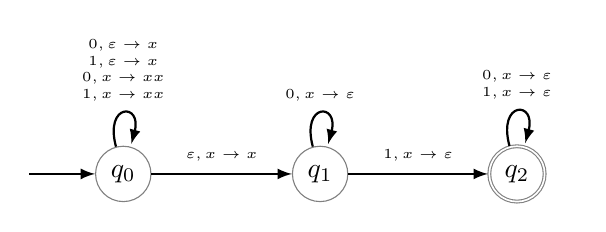
\begin{tikzpicture}[state/.style={circle, draw=black!50, inner sep=0pt, minimum size=20pt},node distance=2.5cm, on grid, auto] 
		\node[state] (q0) {$q_0$};
		\node[state] (q1) [right=of q0] {$q_1$};
		\node[state, accepting] (q2) [right=of q1] {$q_2$};
		\draw[<-, thick] (q0) -- ++(-1.2cm,0);
		\path[->,thick]
			(q0) edge [loop above] node {\tiny\begin{tabular}{c}
				$0,\varepsilon \rightarrow x$ \\
				$1,\varepsilon \rightarrow x$ \\
				$0, x \rightarrow xx$\\
				$1, x \rightarrow xx$\end{tabular}}
			(q0) edge node {\tiny\begin{tabular}{c}$\varepsilon, x \rightarrow x $ \end{tabular}} (q1)
			(q1) edge [loop above] node {\tiny\begin{tabular}{c}$0,x \rightarrow \varepsilon$ \end{tabular}} 
			(q1) edge node {\tiny\begin{tabular}{c}$1, x \rightarrow \varepsilon$\end{tabular}}(q2) 
			(q2) edge [loop above] node {\tiny\begin{tabular}{c}$0,x \rightarrow \varepsilon$ \\
											$1,x \rightarrow \varepsilon$ \end{tabular}} (q2);
	\end{tikzpicture}
	\end{center}
\item[\textbf{b}.]CFG is: \\
		\leavevmode \\
	\setlength\parindent{100pt} 
	$S \rightarrow UV$\\
	$U \rightarrow AB$ \\
	$V \rightarrow A1A \mid A1B \mid A1U \mid B1U \mid U1U$\\
	$A \rightarrow 00^* \mid \varepsilon$\\
	$W \rightarrow 11^* \mid \varepsilon$\\
	\setlength\parindent{0pt} 

Explanation:\\
	\begin{itemize}
		\item The string $S$ is the concatenation of $U$ and $V$.
		\item The string $U$ may consist of any number of 0's and 1's.
		\item The string $V$ may consist of at least one 1 or only one 1.
		\item The string $A$ may consist of at least one zero or more than one zeros
		\item The string $B$ may consist of at least one 1 or more than one 1.
	\end{itemize}
\end{enumerate}
\end{document} 